
%\documentclass[10pt, letterpaper]{article}
\documentclass[10pt, letterpaper]{book}

% package used to set margins, adjust parameters with caution
\usepackage[left = 0.70in, right = 0.70in, top = 1.0in, bottom = 1.0in]{geometry}

%%%%%%%%%%%%%%%%%%%%%%%%%%%%%%%%%%%%%%%%%%%%%%
%%%%%%%%%%%%%%%%%%%%%%%%%%%%%%%%%%%%%%%%%%%%%%

% package used to include special header and footer formatting
\usepackage{fancyhdr}

% package used to include special formatting for image and table captions
\usepackage[small,bf,justification=raggedright,format=hang]{caption}

\usepackage{amscd}
\usepackage{amsfonts}
\usepackage{amsmath}
\usepackage{amssymb}
\usepackage{mathrsfs}
\usepackage{bm}

\usepackage{color}
\usepackage[usenames,dvipsnames]{xcolor}
\usepackage{epsfig}
\usepackage{graphicx}
\usepackage{multicol}
\usepackage{verbatim}
%\usepackage{doublespace}
\usepackage{colortbl}
\usepackage{tcolorbox}

%%%%%%%%%%%%%%%%%%%%%%%%%%%%%%%%%%%%%%%%%%%%%%
%%%%%%%%%%%%%%%%%%%%%%%%%%%%%%%%%%%%%%%%%%%%%%
\renewcommand{\theenumi}{\arabic{enumi}}
\renewcommand{\labelenumi}{\mbox{}\;\theenumi.$\;$}

\renewcommand{\theenumii}{\alph{enumii}}
\renewcommand{\labelenumii}{\mbox{}\;\;\,\theenumii)$\quad$}

\renewcommand{\theenumiii}{\roman{enumiii}}
\renewcommand{\labelenumiii}{\mbox{}\;\;\,\theenumiii)$\quad$}

\renewcommand{\theequation}{\thesection .\arabic{equation}}

\newcounter{theorem}

\newtheorem{example}[theorem]{Example}
\renewcommand{\theexample}{ \thesection .\arabic{example}}

\newtheorem{definition}[theorem]{Definition}
\renewcommand{\thedefinition}{\thesection .\arabic{definition}}

\newtheorem{theorem}[theorem]{Theorem}
\renewcommand{\thetheorem}{\thesection .\arabic{theorem}}

\newtheorem{proposition}[theorem]{Proposition}
\renewcommand{\theproposition}{\thesection .\arabic{proposition}}

\newtheorem{conjecture}[theorem]{Conjecture}
\renewcommand{\theconjecture}{\thesection .\arabic{conjecture}}

\newtheorem{lemma}[theorem]{Lemma}
\renewcommand{\thelemma}{\thesection .\arabic{lemma}}

\newtheorem{corollary}[theorem]{Corollary}
\renewcommand{\thecorollary}{\thesection .\arabic{corollary}}

\newtheorem{remark}[theorem]{Remark}
\renewcommand{\theremark}{\thesection .\arabic{remark}}

\newtheorem{notation}[theorem]{Notation}
\renewcommand{\thenotation}{\thesection .\arabic{notation}}

\renewcommand{\thetable} {\thesection .\arabic{table}}

\renewcommand{\thefigure}{\thesection .\arabic{figure}}

%%%%%%%%%%%%%%%%%%%%%%%%%%%%%%%%%%%%%%%%%%%%%%
%%%%%%%%%%%%%%%%%%%%%%%%%%%%%%%%%%%%%%%%%%%%%%
\newcommand*{\proof}{\noindent {\small P{\scriptsize ROOF}} \quad}
\newcommand*{\proofof}{\noindent {\small P{\scriptsize ROOF OF }}}
\newcommand*{\proofoutline}{\noindent {\small O{\scriptsize UTLINE OF PROOF}} \quad}
\newcommand*{\proofoutlineof}{\noindent {\small O{\scriptsize UTLINE OF PROOF OF }}}
\newcommand*{\qed}{\hfill $\Box$}
\newcommand*{\hdiamond}{\hfill $\Diamond$}

\renewcommand*{\Re}{\mathbb{R}}
\renewcommand*{\d}{\textnormal{d}}
\newcommand{\C}{\mathbb{C}}
\newcommand{\Q}{\mathbb{Q}}
\newcommand{\N}{\mathbb{N}}
\newcommand{\Z}{\mathbb{Z}}
\newcommand{\F}{\mathbb{F}}
\newcommand{\varemptyset}{\varnothing}
\renewcommand{\i}{\textnormal{\bf i}}

\newcommand{\diag}{\textnormal{diag}}
\newcommand{\proj}{\textnormal{proj}}
\newcommand{\rot}{\textnormal{rot}}

\newcommand{\ev}{\textnormal{ev}}
\newcommand{\rank}{\textnormal{rank}}
\renewcommand*{\span}{\textnormal{span}}
\newcommand*{\domain}{\textnormal{domain}}
\newcommand*{\codomain}{\textnormal{codomain}}
\newcommand{\Col}{\textnormal{Col}}
\newcommand{\image}{\textnormal{image}}
\newcommand{\Var}{\textnormal{Var}}
%\newcommand{\Hess}{\textnormal{Hess}}
\newcommand{\Hess}{\nabla^{2}}
\newcommand{\Cov}{\textnormal{Cov}}
\newcommand{\MSE}{\textnormal{MSE}}
\newcommand{\SVar}{\textnormal{SVar}}

\newcommand*{\longhookrightarrow}{\ensuremath{\lhook\joinrel\relbar\joinrel\rightarrow}}

%\newcommand{\Czo}{C([0,1],\Re)}
\newcommand{\Czo}{C[0,1]}

\newcommand{\logisticBetaX}{
	\dfrac{\exp\!\left(\,\beta^{T} \cdot x \,\right)}{1 \,+\, \exp\!\left(\,\beta^{T} \cdot x \,\right)}
}

\newcommand{\oneMinusLogisticBetaX}{
	\dfrac{1}{1 \,+\, \exp\!\left(\,\beta^{T} \cdot x \,\right)}
}

\newcommand{\argmin}{\textnormal{argmin}}
\newcommand{\argmax}{\textnormal{argmax}}

%%%%%%%%%%%%%%%%%%%%%%%%%%%%%%%%%%%%%%%%%%%%%%
%%%%%%%%%%%%%%%%%%%%%%%%%%%%%%%%%%%%%%%%%%%%%%

\begin{document}

%%%%%%%%%%%%%%%%%%%%%%%%%%%%%%%%%%%%%%%%%%%%%%

%\setcounter{page}{1}

\pagestyle{fancy}

\rhead[Study Notes]{Kenneth Chu}
\lhead[Kenneth Chu]{Study Notes}
\chead[]{{\Large\bf Mathematical Theory of the Standard Model of Particle Physics} \\
\vskip 0.1cm \normalsize \today}
\lfoot[]{}
\cfoot[]{}
\rfoot[]{\thepage}

%%%%%%%%%%%%%%%%%%%%%%%%%%%%%%%%%%%%%%%%%%%%%%

          %%%%% ~~~~~~~~~~~~~~~~~~~~ %%%%%

%\mbox{}\vskip 0.0cm
\pagecolor{black}

\begin{titlepage}
\begin{center}
\vspace*{0.8cm}

\resizebox{0.7\linewidth}{!}{\bf\itshape\color{yellow}Mathematical Theory}
\vskip 0.3cm
\textbf{\color{yellow}\fontsize{40}{43}\selectfont\itshape of the}
\vskip 0.2cm
\resizebox{0.8\linewidth}{!}{\bf\itshape\color{yellow}Standard Model}
\vskip 0.3cm
\textbf{\color{yellow}\fontsize{50}{53}\selectfont\itshape of}
\vskip 0.2cm
\resizebox{0.8\linewidth}{!}{\bf\itshape\color{yellow}Particle Physics}
            
\vspace{0.5cm}
\Huge
\textbf{\color{yellow}Kenneth Chu}

\vspace{0.9cm}
%\includegraphics[width=0.99\textwidth]{graphics/090516_standardmodel_2.jpg}
%\includegraphics[width=0.99\textwidth]{graphics/HT_proton_collision_nt_130703_33x16_1600.jpg}
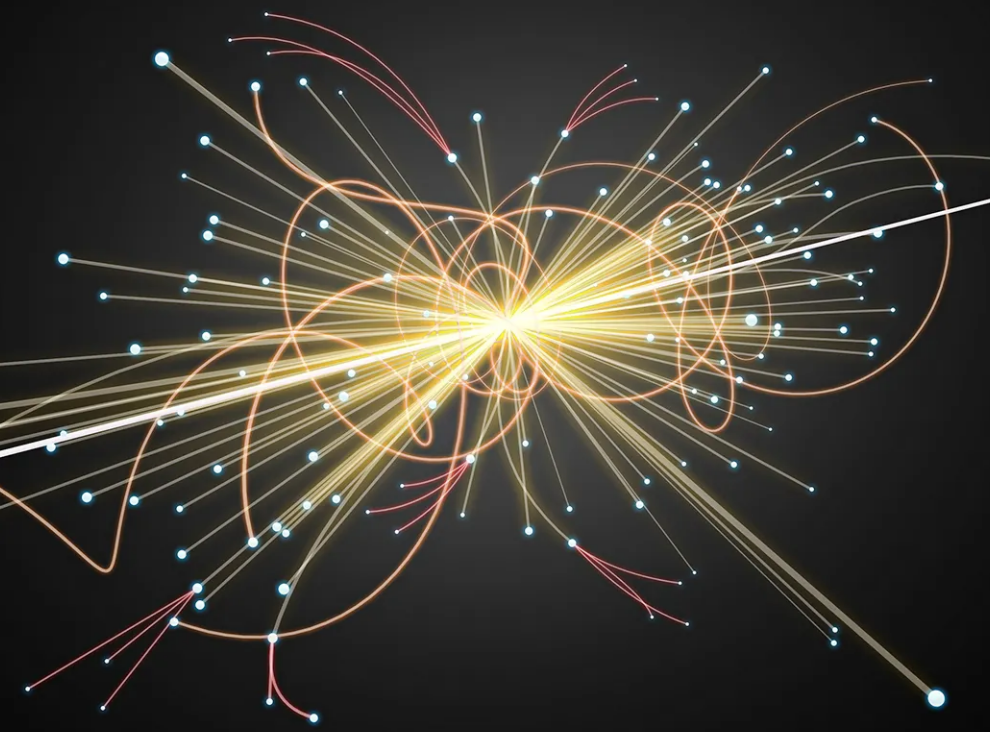
\includegraphics[width=0.90\textwidth]{graphics/lhc-particle-collision-523875355-f.png}
\vspace{-0.2cm}

\Large
{\color{yellow}\today}
            
\end{center}
\end{titlepage}

\pagecolor{white}
%\titlepage

\tableofcontents


          %%%%% ~~~~~~~~~~~~~~~~~~~~ %%%%%

\chapter{Lagrangian mechanics}
\setcounter{theorem}{0}
\setcounter{equation}{0}

%\cite{vanDerVaart1996}
%\cite{Kosorok2008}

%\renewcommand{\theenumi}{\alph{enumi}}
%\renewcommand{\labelenumi}{\textnormal{(\theenumi)}$\;\;$}
\renewcommand{\theenumi}{\roman{enumi}}
\renewcommand{\labelenumi}{\textnormal{(\theenumi)}$\;\;$}

          %%%%% ~~~~~~~~~~~~~~~~~~~~ %%%%%

\begin{definition}[Lagrangian mechanical system, Definition 2.1, \cite{Cortes2017}]
\mbox{}
\vskip 0.1cm
\noindent
A \,\textbf{Lagrangian mechanical system}\, is a pair \,$\left(\,M,\mathscr{L}\,\right)$\,
consisting of a smooth manifold \,$M$ and a smooth $\Re$-valued function
\,$\mathscr{L} : TM \longrightarrow \Re$\,
defined on the tangent bundle \,$TM$ of \,$M$.
The manifold \,$M$ is called the \textbf{configuration space} and
the function \,$\mathscr{L}$\, is called the \textbf{Lagrangian function}
(or simply the \textbf{Lagrangian}) of the system.
\end{definition}

          %%%%% ~~~~~~~~~~~~~~~~~~~~ %%%%%

\vskip 0.5cm
\begin{definition}[Hamilton's principle of least action]
\mbox{}
\vskip 0.1cm
\noindent
Let \,$\left(\,M,\mathscr{L}\,\right)$ be a Lagrangian mechanical system.
The \,\textbf{action}\, of a smooth parametrized curve
\,$\gamma : [\,a, b\,] \longrightarrow M$\,
is defined as
\begin{equation*}
S(\,\gamma\,)
\;\; := \;\;
\int_{a}^{b}
\mathscr{L}(\,\gamma(t)\,)\,\d t.
\end{equation*}
A \,\textbf{motion}\, of the system is a critical point of \,$S$\,
under smooth variations with fixed endpoints.
(This statement is a mathematical formulation of
\textbf{Hamilton's principle of least action},
which should better be called principle of {\color{red}stationary} action.)
\end{definition}

          %%%%% ~~~~~~~~~~~~~~~~~~~~ %%%%%

\vskip 0.5cm
\begin{definition}[Induced coordinate systems]
\mbox{}
\vskip 0.1cm
\noindent
Suppose:
\begin{itemize}
\item
	$\left(\,M,\mathscr{L}\,\right)$ is a Lagrangian mechanical system, with \,$n \,:=\, \dim(M)$, and
\item
	$(x^{1},\ldots,x^{n}) : U \subset M \longrightarrow \Re^{n}$\,
	is a local coordinate system.
\end{itemize}
Then, the \,\textbf{induced coordinate sytem}\, of \,$(x^{1},\ldots,x^{n})$\, is
\,$\left(\,q^{1},\ldots,q^{n},\hat{q}^{\,1},\ldots,\hat{q}^{\,n}\,\right) : \pi^{-1}(U) \longrightarrow \Re^{2n}$\,
given by
\begin{equation*} 
q^{i} \; := \; x^{i} \circ \pi \,:\, \pi^{-1}(U) \,\longrightarrow\, \Re,
\quad\textnormal{and}\quad
\hat{q}^{\,i} \; := \; \d x^{i} \,:\, \pi^{-1}(U) \,\longrightarrow\, \Re\,,
\end{equation*}
where \,$\pi : TM \longrightarrow M$\, is the canoncial projection.
\end{definition}

          %%%%% ~~~~~~~~~~~~~~~~~~~~ %%%%%

\vskip 0.5cm
\begin{remark}[Gradient of the Lagrangian function w.r.t. an induced coordinate system]
\mbox{}
\vskip 0.1cm
\noindent
Note that
\begin{equation*}
\nabla_{(q^{1},\ldots,q^{n},\hat{q}^{\,1},\ldots,\hat{q}^{\,n})}\,\mathscr{L}
\;\; = \;\;
	\left(\,
		\dfrac{\partial\mathscr{L}}{\partial q^{1}}\,,
		\,\ldots\,,
		\dfrac{\partial\mathscr{L}}{\partial q^{n}}\,,
		\dfrac{\partial\mathscr{L}}{\partial \hat{q}^{\,1}}\,,
		\,\ldots\,
		\dfrac{\partial\mathscr{L}}{\partial \hat{q}^{\,n}}
		\,\right)
\; : \;
	\pi^{-1}(U) \; \longrightarrow \; \Re^{2n}
\end{equation*}
The component functions of
\,$\nabla_{(q^{1},\ldots,q^{n},\hat{q}^{\,1},\ldots,\hat{q}^{\,n})}\,\mathscr{L}$\,
appear in the Euler-Lagrange equations,
the ordinary differential equations that determine the motions
of a Lagrangian mechanical system;
see Proposition \ref{EulerLagrangeEquations}.
\end{remark}

          %%%%% ~~~~~~~~~~~~~~~~~~~~ %%%%%

\vskip 0.5cm
\begin{proposition}[Equations of motion, Euler-Lagrangian equations]
\label{EulerLagrangeEquations}
\mbox{}
\vskip 0.1cm
\noindent
A smooth parametrized curve
\,$\gamma : [\,a,b\,] \longrightarrow M$\,
in a Lagrangian mechanical system
\,$\left(\,M,\mathscr{L}\,\right)$\,
is a motion if and only if
\,$\gamma$\,
satisfies the following ordinary differential equations:
\begin{equation*}
\dfrac{\partial\mathscr{L}}{\partial q^{i}}\!\left(\gamma^{\prime}(t)\right)
\; - \;
\dfrac{\d}{\d t}\!\left(\,\dfrac{\partial\mathscr{L}}{\partial \hat{q}^{\,i}}\!\left(\gamma^{\prime}(t)\right)\right)
\;\; = \;\;
0\,,
\end{equation*}
for each \,$i = 1, 2, \,\ldots\, , n \,:=\, \dim(M)$,
each \,$t \in [\,a,b\,]$, and
each induced coordinate system\\
\,$\left(\,q^{1},\ldots,q^{n},\hat{q}^{\,1},\ldots,\hat{q}^{\,n}\,\right)$\,
containing \,$\gamma(t) \in M$.
\end{proposition}
\proof
\begin{equation}\label{VariationVectorField}
\left.\dfrac{\d}{\d s}\right\vert_{s=0} \mathscr{L}\!\left(\gamma_{s}(t)\right)
\;\; = \;\;
	\overset{n}{\underset{i=1}{\sum}}\,\left\{\,
		\dfrac{\partial\mathscr{L}}{\partial q^{i}}\!\left(\gamma^{\prime}_{0}(t)\right)
		\cdot
		\left.\dfrac{\d}{\d s}\right\vert_{s=0} q^{i}(\gamma^{\prime}_{s}(t))
		\, + \,
		\dfrac{\partial\mathscr{L}}{\partial\hat{q}^{\,i}}\!\left(\gamma^{\prime}_{0}(t)\right)
		\cdot
		\left.\dfrac{\d}{\d s}\right\vert_{s=0} \hat{q}^{\,i}(\gamma^{\prime}_{s}(t))
		\,\right\}
\end{equation}
Now, observe that
\begin{eqnarray*}
\left.\dfrac{\d}{\d s}\right\vert_{s=0} \hat{q}^{\,i}(\gamma^{\prime}_{s}(t))
& = &
	\left.\dfrac{\d}{\d s}\right\vert_{s=0} \d x^{i}(\gamma^{\prime}_{s}(t))
\;\; = \;\;
	\left.\dfrac{\d}{\d s}\right\vert_{s=0} \, \dfrac{\d}{\d t}\,(x^{i}\circ\gamma_{s})(t)
\;\; = \;\;
	\dfrac{\d}{\d t}\; \left.\dfrac{\d}{\d s}\right\vert_{s=0} \, (x^{i}\circ\gamma_{s})(t)
\\
& = &
	\overset{{\color{white}1}}{\dfrac{\d}{\d t}}\, W^{i}(t),
\end{eqnarray*}
where
\,$W(t) \,:=\, \left.\dfrac{\d}{\d s}\right\vert_{s=0} \gamma_{s}(t) \,\in\, T_{\gamma(t)}M$\,
is the variation vector field defined along \,$\gamma$.
Hence,
\begin{eqnarray*}
\dfrac{\partial\mathscr{L}}{\partial\hat{q}^{\,i}}\!\left(\gamma^{\prime}_{0}(t)\right)
\cdot
\left.\dfrac{\d}{\d s}\right\vert_{s=0} \hat{q}^{\,i}(\gamma^{\prime}_{s}(t))
& = &
	\dfrac{\partial\mathscr{L}}{\partial\hat{q}^{\,i}}\!\left(\gamma^{\prime}_{0}(t)\right)
	\cdot
	\dfrac{\d}{\d t}\, W^{i}(t)	
\\
& = &
	\dfrac{\d}{\d t}\!\left(\,
		\dfrac{\partial\mathscr{L}}{\partial\hat{q}^{\,i}}\!\left(\gamma^{\prime}_{0}(t)\right)
		\cdot
		W^{i}(t)
		\right)
	\, - \,
	\dfrac{\d}{\d t}\!\left(\,
		\dfrac{\partial\mathscr{L}}{\partial\hat{q}^{\,i}}\!\left(\gamma^{\prime}_{0}(t)\right)
		\right)	
	\cdot
	W^{i}(t)
\end{eqnarray*}
Substituting the above into \eqref{VariationVectorField} yields:
\begin{eqnarray*}
&&
	\left.\dfrac{\d}{\d s}\right\vert_{s=0} \mathscr{L}\!\left(\gamma_{s}(t)\right)
\\
& = &
	\overset{n}{\underset{i=1}{\sum}}\,\left\{\,
		\dfrac{\partial\mathscr{L}}{\partial q^{i}}\!\left(\gamma^{\prime}_{0}(t)\right)
		\cdot
		\left.\dfrac{\d}{\d s}\right\vert_{s=0} q^{i}(\gamma^{\prime}_{s}(t))
		\, + \,
		\dfrac{\partial\mathscr{L}}{\partial\hat{q}^{\,i}}\!\left(\gamma^{\prime}_{0}(t)\right)
		\cdot
		\left.\dfrac{\d}{\d s}\right\vert_{s=0} \hat{q}^{\,i}(\gamma^{\prime}_{s}(t))
		\,\right\}
\\
& = &
	\overset{n}{\underset{i=1}{\sum}}\,\left\{\,
		\dfrac{\partial\mathscr{L}}{\partial q^{i}}\!\left(\gamma^{\prime}(t)\right)
		\cdot
		\left.\dfrac{\d}{\d s}\right\vert_{s=0} x^{i}\circ\pi(\gamma^{\prime}_{s}(t))
		\, - \,
		\dfrac{\d}{\d t}\!\left(\,
			\dfrac{\partial\mathscr{L}}{\partial\hat{q}^{\,i}}\!\left(\gamma^{\prime}(t)\right)
			\right)	
		\cdot
		W^{i}(t)
		\,\right\}
	\; + \;
	\dfrac{\d}{\d t}\!\left(\,
		\overset{n}{\underset{i=1}{\sum}}\;
		\dfrac{\partial\mathscr{L}}{\partial\hat{q}^{\,i}}\!\left(\gamma^{\prime}(t)\right)
		\cdot
		W^{i}(t)
		\right)
\\
& = &
	\overset{n}{\underset{i=1}{\sum}}\,\left\{\,
		\dfrac{\partial\mathscr{L}}{\partial q^{i}}\!\left(\gamma^{\prime}(t)\right)
		\cdot
		\left.\dfrac{\d}{\d s}\right\vert_{s=0} x^{i}\circ\gamma_{s}(t)
		\, - \,
		\dfrac{\d}{\d t}\!\left(\,
			\dfrac{\partial\mathscr{L}}{\partial\hat{q}^{\,i}}\!\left(\gamma^{\prime}(t)\right)
			\right)	
		\cdot
		W^{i}(t)
		\,\right\}
	\; + \;
	f^{\prime}(t)
\\
& = &
	\overset{n}{\underset{i=1}{\sum}}\,\left\{\;
		\dfrac{\partial\mathscr{L}}{\partial q^{i}}\!\left(\gamma^{\prime}(t)\right)
		\, - \,
		\dfrac{\d}{\d t}\!\left(\,
			\dfrac{\partial\mathscr{L}}{\partial\hat{q}^{\,i}}\!\left(\gamma^{\prime}(t)\right)
			\right)
		\right\}
	\cdot
	W^{i}(t)
	\; + \;
	f^{\prime}(t)
\end{eqnarray*}
where
\begin{equation*}
f(t)
\;\; := \;\;
	\overset{n}{\underset{i=1}{\sum}}\;
	\dfrac{\partial\mathscr{L}}{\partial\hat{q}^{\,i}}\!\left(\gamma^{\prime}(t)\right)
	\cdot
	W^{i}(t)\,,
\quad
\textnormal{for \,$t \in [\,a,b\,]$}
\end{equation*}

\vskip 0.5cm
\noindent
\textbf{Claim 1:}
\vskip 0.1cm
\noindent
$f : [\,a,b\,] \longrightarrow \Re$\, is globally well-defined on \,$[\,a,b\,]$;\,
more precisely, the local definition of \,$f$\, above is in fact
independent of the choice of the local coordinate system.
Furthermore, \,$f(a) = f(b) = 0$.
\vskip 0.2cm
\noindent
Proof of Claim 1: \quad
\begin{equation*}
T^{\textnormal{ver}}_{\gamma(t)}(TM)
\;\; := \;\;
	\textnormal{ker}\!\left(\,\d\pi\vert_{\gamma(t)}\,\right)
\;\; \subset \;\;
	T_{\gamma(t)}(TM).
\end{equation*}
\begin{eqnarray*}
&&
	\left.\dfrac{\d}{\d s}\right\vert_{s=0} S\!\left(\gamma_{s}\right)
\\
& = &
	\left.\dfrac{\d}{\d s}\right\vert_{s=0}\; \int_{a}^{b}\,\mathscr{L}\!\left(\gamma_{s}(t)\right)\d t
\;\; = \;\;
	\int_{a}^{b}\left(\left.\dfrac{\d}{\d s}\right\vert_{s=0}\,\mathscr{L}\!\left(\gamma_{s}(t)\right)\right)\d t
\\
& = &
	\int_{a}^{b}\left(\;
		\overset{n}{\underset{i=1}{\sum}}\,\left\{\;
			\dfrac{\partial\mathscr{L}}{\partial q^{i}}\!\left(\gamma^{\prime}(t)\right)
			\, - \,
			\dfrac{\d}{\d t}\!\left(\,
				\dfrac{\partial\mathscr{L}}{\partial\hat{q}^{\,i}}\!\left(\gamma^{\prime}(t)\right)
				\right)
			\right\}
		\cdot
		W^{i}(t)
		\; + \;
		f^{\prime}(t)
		\right)\d t
\\
& = &
	\int_{a}^{b}\left(\;
		\overset{n}{\underset{i=1}{\sum}}\,\left\{\;
			\dfrac{\partial\mathscr{L}}{\partial q^{i}}\!\left(\gamma^{\prime}(t)\right)
			\, - \,
			\dfrac{\d}{\d t}\!\left(\,
				\dfrac{\partial\mathscr{L}}{\partial\hat{q}^{\,i}}\!\left(\gamma^{\prime}(t)\right)
				\right)
			\right\}
		\cdot
		W^{i}(t)
		\right)\d t
	\; + \;
	\left(\, f(b) \overset{{\color{white}1}}{-} f(a) \,\right)
\\
& = &
	\int_{a}^{b}\left(\;
		\overset{n}{\underset{i=1}{\sum}}\,\left\{\;
			\dfrac{\partial\mathscr{L}}{\partial q^{i}}\!\left(\gamma^{\prime}(t)\right)
			\, - \,
			\dfrac{\d}{\d t}\!\left(\,
				\dfrac{\partial\mathscr{L}}{\partial\hat{q}^{\,i}}\!\left(\gamma^{\prime}(t)\right)
				\right)
			\right\}
		\cdot
		W^{i}(t)
		\right)\d t
\end{eqnarray*}

\qed

          %%%%% ~~~~~~~~~~~~~~~~~~~~ %%%%%

          %%%%% ~~~~~~~~~~~~~~~~~~~~ %%%%%

          %%%%% ~~~~~~~~~~~~~~~~~~~~ %%%%%



          %%%%% ~~~~~~~~~~~~~~~~~~~~ %%%%%

\section{Symplectic geometry}
\setcounter{theorem}{0}
\setcounter{equation}{0}

%\cite{vanDerVaart1996}
%\cite{Kosorok2008}

%\renewcommand{\theenumi}{\alph{enumi}}
%\renewcommand{\labelenumi}{\textnormal{(\theenumi)}$\;\;$}
\renewcommand{\theenumi}{\roman{enumi}}
\renewcommand{\labelenumi}{\textnormal{(\theenumi)}$\;\;$}

          %%%%% ~~~~~~~~~~~~~~~~~~~~ %%%%%

\begin{theorem}
\mbox{}
\vskip 0.2cm
\noindent
Suppose $(M,\omega)$ is symplectic manifold. Then,
\begin{enumerate}
\item
	The set $C^{\infty}(M)$ of smooth $\Re$-valued functions on $M$
	forms a Lie algebra under the Poisson bracket.
\item
	The set $V^{\textnormal{LH}}(M)$ of locally Hamiltonian vector fields defined on $M$
	forms a Lie algebra under the Lie bracket, and
	the set $V^{\textnormal{H}}(M) \subset V^{\textnormal{LH}}(M)$ of (globally) Hamiltonian vector fields
	is a Lie algebra ideal of $V^{\textnormal{LH}}(M)$.
\item
	For each $f \in C^{\infty}(M)$, let $X_{f} \in V^{\textnormal{H}}(M)$ denotes the Hamiltonian vector field generated by $f$.
	Then, the map $C^{\infty}(M) \longrightarrow V^{\textnormal{H}}(M)$ is a Lie algebra homomorphism
	with kernel being the set of constant $\Re$-valued functions on $M$.
	In particular, we have the following Lie-algebra isomorphism
	\begin{equation*}
	V^{\textnormal{H}}(M) \;\; \cong \;\; C^{\infty}(M) \,/\, \Re.
	\end{equation*}
\end{enumerate}
\end{theorem}

          %%%%% ~~~~~~~~~~~~~~~~~~~~ %%%%%

          %%%%% ~~~~~~~~~~~~~~~~~~~~ %%%%%



          %%%%% ~~~~~~~~~~~~~~~~~~~~ %%%%%

%\clearpage
%\appendix
%\input{tex/z-exercises}
%
          %%%%% ~~~~~~~~~~~~~~~~~~~~ %%%%%

\section{Technical lemmas}
\setcounter{theorem}{0}
\setcounter{equation}{0}

%\cite{vanDerVaart1996}
%\cite{Kosorok2008}

%\renewcommand{\theenumi}{\alph{enumi}}
%\renewcommand{\labelenumi}{\textnormal{(\theenumi)}$\;\;$}
\renewcommand{\theenumi}{\roman{enumi}}
\renewcommand{\labelenumi}{\textnormal{(\theenumi)}$\;\;$}

          %%%%% ~~~~~~~~~~~~~~~~~~~~ %%%%%

\begin{lemma}\label{lemma:MonotoneFunctionsAreMeasurable}
\mbox{}\vskip 0.1cm
\noindent
Suppose $B \subset \Re$ be a Borel measurable subset of \,$\Re$, and
$f : B \longrightarrow \Re$ is an $\Re$-valued function defined on $B$.
If $f$ is monotone, then $f$ is Borel measurable.
\end{lemma}
\proof
Suppose that $(\Omega,\mathcal{A})$ is a measurable space and
$f : \Omega \longrightarrow \Re$ is an $\Re$-valued function defined on $\Omega$.
Let $\mathcal{O}$ denote the Borel $\sigma$-algebra of $\Re$.
Recall that $f$ is said to be $(\mathcal{A},\mathcal{O})$-measurable if
$f^{-1}\!\left(\,(-\infty,\overset{{\color{white}-}}{y}\,]\,\right) \in \mathcal{A}$,
for each $y \in \Re$.

\vskip 0.3cm
\noindent
Now we specialize to the scenario of the present Lemma, namely that
$(\Omega,\mathcal{A}) = (\Re,\mathcal{O})$.

\vskip 0.3cm
\noindent
We give the proof only for the case where $f$ is nondecreasing.
The proof for the case where $f$ is nonincreasing in similar.
Now, for nondecreasing $f$, the present Lemma follows immediately
from Claim 1 below, since \,$\varemptyset$, \,$B = B \cap (-\infty,\infty)$,
\,$B \cap (-\infty,x\,)$,\, and \,$B \cap (-\infty,x\,]$\, are measurable, for every $x\in\Re$.

%\vskip 0.5cm
%\noindent
%\textbf{Claim 1:}\quad
%For any $x \in B$,\;
%$x \,\in\, f^{-1}\!\left(\,(\,-\infty,\overset{{\color{white}-}}{y}\,]\,\right)$\,
%\,$\Longrightarrow$\;
%$B \cap (-\infty,x\,] \,\subset\, f^{-1}\!\left(\,(\,-\infty,\overset{{\color{white}-}}{y}\,]\,\right)$
%\vskip 0.1cm
%\noindent
%Proof of Claim 1:\;\;
%First, note that $x \,\in\, f^{-1}\!\left(\,(\,-\infty,\overset{{\color{white}-}}{y}\,]\,\right)$
%\;$\Longleftrightarrow$\; $f(x) \leq y$.
%Now, since $f$ is nondecreasing, we see that
%$\xi \in B \cap (-\infty,x\,]$ \;$\Longrightarrow$\; $f(\xi) \leq f(x) \leq y$
%\;$\Longrightarrow$\; $\xi \,\in\, f^{-1}\!\left(\,(\,-\infty,\overset{{\color{white}-}}{y}\,]\,\right)$.
%This shows that indeed \,$B \cap (-\infty,x\,] \,\subset\, f^{-1}\!\left(\,(\,-\infty,\overset{{\color{white}-}}{y}\,]\,\right)$,\,
%and completes the proof of Claim 1.

\vskip 0.5cm
\noindent
\textbf{Claim 1:}\quad
$f^{-1}\!\left(\,(\,-\infty,\overset{{\color{white}-}}{y}\,]\,\right)$\,
is either \,$\varemptyset$, \,$B \cap (-\infty,\infty)$, \,$B \cap (-\infty,x\,)$,\, or \,$B \cap (-\infty,x\,]$,\, for some $x\in\Re$.
\vskip 0.1cm
\noindent
Proof of Claim 1:\;\;
First, note that
\begin{eqnarray*}
y \,\geq\, \underset{\xi \in B}{\sup}\left\{\;\overset{{\color{white}.}}{f}(\xi)\;\right\} \,\in\, \Re\cup\{\,+\infty\,\}
& \Longrightarrow &
	f^{-1}\!\left(\,(\,-\infty,\overset{{\color{white}-}}{y}\,]\,\right) \,=\, B \cap (-\infty,\infty) \,=\, B\,,
	\quad
	\textnormal{and}
\\
y \,<\, \underset{\xi \in B}{\inf}\left\{\;\overset{{\color{white}.}}{f}(\xi)\;\right\} \,\in\, \Re\cup\{\,-\infty\,\}
& \Longrightarrow &
	f^{-1}\!\left(\,(\,-\infty,\overset{{\color{white}-}}{y}\,]\,\right) \,=\, \varemptyset\,.
\end{eqnarray*}
Next, we consider the case where
\;$-\infty \,\leq\, \underset{\xi \in B}{\inf}\left\{\;\overset{{\color{white}.}}{f}(\xi)\;\right\}
\;\leq\; y \,<\, \underset{\xi \in B}{\sup}\left\{\;\overset{{\color{white}.}}{f}(\xi)\;\right\} \,\leq\, +\infty$.
Let
\begin{equation*}
x \;\; := \;\; \sup\,f^{-1}\!\left(\,(-\infty,\overset{{\color{white}-}}{y}\,]\,\right) \;\; \in \;\; \Re\cup\{\,+\infty\,\}.
\end{equation*}
Then, we claim have
\begin{equation*}
B \cap (-\infty,x\,)
\;\;\subset\;\;
	f^{-1}\!\left(\,(-\infty,\overset{{\color{white}-}}{y}\,]\,\right)
\;\;\subset\;\;
	B \cap (-\infty,x\,].
\end{equation*}
Indeed, note that
$x \,:=\, \sup\,f^{-1}\!\left(\,(-\infty,\overset{{\color{white}-}}{y}\,]\,\right)$
trivially implies that
$f^{-1}\!\left(\,(-\infty,\overset{{\color{white}-}}{y}\,]\,\right) \subset\,B \cap (-\infty,x\,]$.
On the other hand, by definition of the supremum, there exists a sequence
$\{\,\xi_{n}\,\}_{n\in\N} \,\subset\, f^{-1}\!\left(\,(-\infty,\overset{{\color{white}-}}{y}\,]\,\right)$
such that $\xi_{n} \uparrow x$.
Since $f$ is nondecreasing, we see that $f(\xi_{n})$ is also nondecreasing.
Thus, the limit $\underset{n\rightarrow\infty}{\lim}f(\xi_{n})$ exists and $\underset{n\rightarrow\infty}{\lim}f(\xi_{n}) \,\leq\, y$.
Therefore,
\begin{eqnarray*}
\xi \in B \cap (-\infty,x\,)
&\Longrightarrow&
	\xi \,<\, x
\;\;\Longrightarrow\;\;
	\exists \;\; m\,\in\,\N \;\;\textnormal{such that}\;\; \xi \,\leq\, \xi_{m} \,\leq\, x
\\
&\Longrightarrow&
	f(\xi) \,\leq\, f(\xi_{m}) \,\leq\, \underset{n\rightarrow\infty}{\lim}f(\xi_{n}) \,\leq\, y
\;\;\Longrightarrow\;\;
	\xi \in f^{-1}\!\left(\,(-\infty,\overset{{\color{white}-}}{y}\,]\,\right),
\end{eqnarray*}
which proves that \,$B \cap (-\infty,x\,) \,\subset\, f^{-1}\!\left(\,(-\infty,\overset{{\color{white}-}}{y}\,]\,\right)$.
This completes the proof of Claim 1, as well as that of the present Lemma.
\qed

          %%%%% ~~~~~~~~~~~~~~~~~~~~ %%%%%

\begin{lemma}\label{lemma:nondecreasingLeftContinuous}
\mbox{}\vskip 0.1cm
\noindent
Suppose:
\begin{itemize}
\item
	$(\,a,b\,], (\,c,d\,] \subset \Re$ are intervals in \,$\Re$.
\item
	$\phi : (\,a,b\,] \longrightarrow (\,c,d\,]$ is a nondecreasing and left-continuous
	$\Re$-valued function mapping from $(\,a,b\,]$ {\color{red}onto} $(\,c,d\,]$.
	Note that, since $\phi$ is nondecreasing and left-continuous, we have:
	\begin{equation*}
	c \; = \; \underset{\xi\,\rightarrow\,a^{+}}{\lim}\phi(\xi) \; \in \; \Re\cup\{\,-\infty\,\}
	\quad\textnormal{and}\quad
	d \; = \; \underset{\xi\,\rightarrow\,b^{-}}{\lim}\phi(\xi) \; = \; \phi(b) \; \in \; \Re
	\end{equation*}
\end{itemize}
Define \;$\psi : (\,c,d\,] \longrightarrow (\,a,b\,]$\; as follows:
\begin{equation*}
\psi(y)
\;\; := \;\;
	\sup\left\{\;
		x \in (\,a,b\,]
	\,\;\left\vert\;\,
		\overset{{\color{white}.}}{\phi}(x) \leq y
	\right.
	\;\right\}.
\end{equation*}
Then,
\begin{enumerate}
\item
	$\psi$ is nondecreasing and measurable.
\item
	$\phi$ and $\psi$ satisfy:\quad
	$\phi(x) \,\leq\, y \;\; \Longleftrightarrow \;\; x \,\leq\, \psi(y)$,\;\;
	for each \;$x \in (\,a,b\,]$\; and \;$y \in (\,c,d\,]$.
\end{enumerate}
\end{lemma}
\proof
\begin{enumerate}
\item
	We first show that $\psi$ is nondecreasing.
	Suppose $y_{1} \leq y_{2}$. Then, for each $x \in (\,a,b\,]$, we have
	$\phi(x) \leq y_{1}$ $\Longrightarrow$ $\phi(x) \leq y_{2}$.
	Hence
	\begin{equation*}
	\left\{\;
		x \in (\,a,b\,]
		\,\;\left\vert\;\,
			\overset{{\color{white}.}}{\phi}(x) \leq y_{1}
		\right.
		\;\right\}
	\;\; \subset \;\;
	\left\{\;
		x \in (\,a,b\,]
		\,\;\left\vert\;\,
			\overset{{\color{white}.}}{\phi}(x) \leq y_{2}
		\right.
		\;\right\},
	\end{equation*}
	which implies
	\begin{equation*}
	\psi(y_{1}) \; := \;
	\sup\left\{\;
		x \in (\,a,b\,]
		\,\;\left\vert\;\,
			\overset{{\color{white}.}}{\phi}(x) \geq y_{2}
		\right.
		\;\right\}
	\;\; \leq \;\;
	\sup\left\{\;
		x \in (\,a,b\,]
		\,\;\left\vert\;\,
			\overset{{\color{white}.}}{\phi}(x) \geq y_{1}
		\right.
		\;\right\}
	\; =: \; \psi(y_{2})
	\end{equation*}
	Thus $\psi$ is indeed nondecreasing.
	Measurability of $\psi$ then follows at once from Lemma \ref{lemma:MonotoneFunctionsAreMeasurable}.
\item
	\textbf{\underline{(\,$\Longrightarrow$\,)}}\quad
	$\phi(x) \leq y
	\;\;\Longrightarrow\;\;
		x \in \left\{\,\xi\in(\,a,b\,] \;\left\vert\; \phi(\xi) \overset{{\color{white}.}}{\leq} y\right.\,\right\}
	\;\; \Longrightarrow \;\;
		x \leq \sup\left\{\,\xi\in(\,a,b\,] \;\left\vert\; \phi(\xi) \overset{{\color{white}.}}{\leq} y\right.\,\right\} =: \psi(y)$.

	\vskip 0.2cm
	\noindent
	\textbf{\underline{(\,$\Longleftarrow$\,)}}\quad
	Suppose \;$a \,<\, x \,\leq\, \psi(y) \,\leq\, b$.\;
	Let \;$\delta \,:=\, \psi(y) \,-\, x \,\geq\, 0$. Then,
	\begin{equation*}
	x + \delta \;\;=\;\; \psi(y) \;\;:=\;\; \sup\left\{\,\xi\in(\,a,b\,] \;\left\vert\; \phi(\xi) \overset{{\color{white}.}}{\leq} y\right.\,\right\}.
	\end{equation*}
	Hence, there exists a nondecreasing sequence
	$\xi_{n} \in \left\{\,\xi\in(\,a,b\,] \;\left\vert\; \phi(\xi) \overset{{\color{white}.}}{\leq} y\right.\,\right\}$
	such that $\xi_{n} \uparrow (x+\delta)$.
	Since $\phi$ is {\color{red}nondecreasing and left-continuous}, we see that $\phi(\xi_{n}) \uparrow \phi(x+\delta)$.
	Since $\phi$ is nondecreasing and $\delta \geq 0$, we therefore have
	\begin{equation*}
	\phi(x) \;\;\leq\;\; \phi(x+\delta) \;\;=\;\; \underset{n\rightarrow\infty}{\lim}\,\phi(\xi_{n}) \;\;\leq\;\; y.
	\end{equation*}
\end{enumerate}
\qed

          %%%%% ~~~~~~~~~~~~~~~~~~~~ %%%%%

\begin{lemma}\label{lemma:nondecreasingRightContinuous}
\mbox{}\vskip 0.1cm
\noindent
Suppose:
\begin{itemize}
\item
	$[\,a,b\,), [\,c,d\,) \subset \Re$ are intervals in \,$\Re$.
\item
	$\phi : [\,a,b\,) \longrightarrow [\,c,d\,)$ is a nondecreasing and right-continuous
	$\Re$-valued function mapping from $[\,a,b\,)$ {\color{red}onto} $[\,c,d\,)$.
	Note that, since $\phi$ is nondecreasing and right-continuous, we have:
	\begin{equation*}
	c \; = \; \underset{\xi\,\rightarrow\,a^{+}}{\lim}\phi(\xi) \; = \; \phi(a) \; \in \; \Re
	\quad\textnormal{and}\quad
	d \; = \; \underset{\xi\,\rightarrow\,b^{-}}{\lim}\phi(\xi) \; \in \; \Re\cup\{\,+\infty\,\}
	\end{equation*}
\end{itemize}
Define \;$\psi : [\,c,d\,) \longrightarrow [\,a,b\,)$\; as follows:
\begin{equation*}
\psi(y)
\;\; := \;\;
	\inf\left\{\;
		x \in [\,a,b\,)
	\,\;\left\vert\;\,
		\overset{{\color{white}.}}{\phi}(x) \geq y
	\right.
	\;\right\}.
\end{equation*}
Then,
\begin{enumerate}
\item
	$\psi$ is nondecreasing and measurable.
\item
	$\phi$ and $\psi$ satisfy:\quad
	$\phi(x) \,\geq\, y \;\; \Longleftrightarrow \;\; x \,\geq\, \psi(y)$,\;\;
	for each \;$x \in [\,a,b\,)$\; and \;$y \in [\,c,d\,)$.
\end{enumerate}
\end{lemma}
\proof
\begin{enumerate}
\item
	We first show that $\psi$ is nondecreasing.
	Suppose $y_{1} \leq y_{2}$. Then, for each $x \in [\,a,b\,)$, we have
	$\phi(x) \geq y_{2}$ $\Longrightarrow$ $\phi(x) \geq y_{1}$.
	Hence
	\begin{equation*}
	\left\{\;
		x \in [\,a,b\,)
		\,\;\left\vert\;\,
			\overset{{\color{white}.}}{\phi}(x) \geq y_{1}
		\right.
		\;\right\}
	\;\; \supset \;\;
	\left\{\;
		x \in [\,a,b\,)
		\,\;\left\vert\;\,
			\overset{{\color{white}.}}{\phi}(x) \geq y_{2}
		\right.
		\;\right\},
	\end{equation*}
	which implies
	\begin{equation*}
	\psi(y_{1}) \; := \;
	\inf\left\{\;
		x \in [\,a,b\,)
		\,\;\left\vert\;\,
			\overset{{\color{white}.}}{\phi}(x) \geq y_{1}
		\right.
		\;\right\}
	\;\; \leq \;\;
	\inf\left\{\;
		x \in [\,a,b\,)
		\,\;\left\vert\;\,
			\overset{{\color{white}.}}{\phi}(x) \geq y_{2}
		\right.
		\;\right\}
	\; =: \; \psi(y_{2})
	\end{equation*}
	Thus $\psi$ is indeed nondecreasing.
	Measurability of $\psi$ then follows at once from Lemma \ref{lemma:MonotoneFunctionsAreMeasurable}.
\item
	\textbf{\underline{(\,$\Longrightarrow$\,)}}\quad
	$\phi(x) \geq y
	\;\;\Longrightarrow\;\;
		x \in \left\{\,\xi\in[\,a,b\,) \;\left\vert\; \phi(\xi) \overset{{\color{white}.}}{\geq} y\right.\,\right\}
	\;\; \Longrightarrow \;\;
		x \geq \inf\left\{\,\xi\in[\,a,b\,) \;\left\vert\; \phi(\xi) \overset{{\color{white}.}}{\geq} y\right.\,\right\} =: \psi(y)$.

	\vskip 0.2cm
	\noindent
	\textbf{\underline{(\,$\Longleftarrow$\,)}}\quad
	Suppose \;$a \,\leq\, \psi(y) \,\leq\, x \,<\, b$.\;
	Let \;$\delta \,:=\, x \,-\, \psi(y) \,\geq\, 0$. Then,
	\begin{equation*}
	x - \delta \;\;=\;\; \psi(y) \;\;:=\;\; \inf\left\{\,\xi\in[\,a,b\,) \;\left\vert\; \phi(\xi) \overset{{\color{white}.}}{\geq} y\right.\,\right\}.
	\end{equation*}
	Hence, there exists a nonincreasing sequence
	$\xi_{n} \in \left\{\,\xi\in[\,a,b\,) \;\left\vert\; \phi(\xi) \overset{{\color{white}.}}{\geq} y\right.\,\right\}$
	such that $\xi_{n} \downarrow (x-\delta)$.
	Since $\phi$ is {\color{red}nondecreasing and right-continuous}, we see that $\phi(\xi_{n}) \downarrow \phi(x-\delta)$.
	Since $\phi$ is nondecreasing and $\delta \geq 0$, we therefore have
	\begin{equation*}
	\phi(x) \;\;\geq\;\; \phi(x-\delta) \;\;=\;\; \underset{n\rightarrow\infty}{\lim}\,\phi(\xi_{n}) \;\;\geq\;\; y.
	\end{equation*}
\end{enumerate}
\qed

          %%%%% ~~~~~~~~~~~~~~~~~~~~ %%%%%

\begin{lemma}\label{lemma:nonincreasingLeftContinuous}
\mbox{}\vskip 0.1cm
\noindent
Suppose:
\begin{itemize}
\item
	$(\,a,b\,], (\,c,d\,] \subset \Re$ are intervals in \,$\Re$.
\item
	$\phi : (\,a,b\,] \longrightarrow (\,c,d\,]$ is a nonincreasing and left-continuous
	$\Re$-valued function mapping from $(\,a,b\,]$ {\color{red}onto} $(\,c,d\,]$.
	Note that, since $\phi$ is nonincreasing and left-continuous, we have:
	\begin{equation*}
	c \; = \; \underset{\xi\,\rightarrow\,a^{+}}{\lim}\phi(\xi) \; \in \; \Re\cup\{\,-\infty\,\}
	\quad\textnormal{and}\quad
	d \; = \; \underset{\xi\,\rightarrow\,b^{-}}{\lim}\phi(\xi) \; = \; \phi(b) \; \in \; \Re
	\end{equation*}
\end{itemize}
Define \;$\psi : (\,c,d\,] \longrightarrow (\,a,b\,]$\; as follows:
\begin{equation*}
\psi(y)
\;\; := \;\;
	\sup\left\{\;
		x \in (\,a,b\,]
	\,\;\left\vert\;\,
		\overset{{\color{white}.}}{\phi}(x) \geq y
	\right.
	\;\right\}.
\end{equation*}
Then,
\begin{enumerate}
\item
	$\psi$ is nonincreasing and measurable.
\item
	$\phi$ and $\psi$ satisfy:\quad
	$\phi(x) \,\geq\, y \;\; \Longleftrightarrow \;\; x \,\leq\, \psi(y)$,\;\;
	for each \;$x \in (\,a,b\,]$\; and \;$y \in (\,c,d\,]$.
\end{enumerate}
\end{lemma}
\proof
\begin{enumerate}
\item
	We first show that $\psi$ is nonincreasing.
	Suppose $y_{1} \leq y_{2}$. Then, for each $x \in (\,a,b\,]$, we have
	$\phi(x) \geq y_{2}$ $\Longrightarrow$ $\phi(x) \geq y_{1}$.
	Hence
	\begin{equation*}
	\left\{\;
		x \in (\,a,b\,]
		\,\;\left\vert\;\,
			\overset{{\color{white}.}}{\phi}(x) \geq y_{1}
		\right.
		\;\right\}
	\;\; \supset \;\;
	\left\{\;
		x \in (\,a,b\,]
		\,\;\left\vert\;\,
			\overset{{\color{white}.}}{\phi}(x) \geq y_{2}
		\right.
		\;\right\},
	\end{equation*}
	which implies
	\begin{equation*}
	\psi(y_{1}) \; := \;
	\sup\left\{\;
		x \in (\,a,b\,]
		\,\;\left\vert\;\,
			\overset{{\color{white}.}}{\phi}(x) \geq y_{2}
		\right.
		\;\right\}
	\;\; \geq \;\;
	\sup\left\{\;
		x \in (\,a,b\,]
		\,\;\left\vert\;\,
			\overset{{\color{white}.}}{\phi}(x) \geq y_{1}
		\right.
		\;\right\}
	\; =: \; \psi(y_{2})
	\end{equation*}
	Thus $\psi$ is indeed nonincreasing.
	Measurability of $\psi$ then follows at once from Lemma \ref{lemma:MonotoneFunctionsAreMeasurable}.
\item
	\textbf{\underline{(\,$\Longrightarrow$\,)}}\quad
	$\phi(x) \geq y
	\;\;\Longrightarrow\;\;
		x \in \left\{\,\xi\in(\,a,b\,] \;\left\vert\; \phi(\xi) \overset{{\color{white}.}}{\geq} y\right.\,\right\}
	\;\; \Longrightarrow \;\;
		x \leq \sup\left\{\,\xi\in(\,a,b\,] \;\left\vert\; \phi(\xi) \overset{{\color{white}.}}{\geq} y\right.\,\right\} =: \psi(y)$.

	\vskip 0.2cm
	\noindent
	\textbf{\underline{(\,$\Longleftarrow$\,)}}\quad
	Suppose \;$a \,<\, x \,\leq\, \psi(y) \,\leq\, b$.\;
	Let \;$\delta \,:=\, \psi(y) \,-\, x \,\geq\, 0$. Then,
	\begin{equation*}
	x + \delta \;\;=\;\; \psi(y) \;\;:=\;\; \sup\left\{\,\xi\in(\,a,b\,] \;\left\vert\; \phi(\xi) \overset{{\color{white}.}}{\geq} y\right.\,\right\}.
	\end{equation*}
	Hence, there exists a nondecreasing sequence
	$\xi_{n} \in \left\{\,\xi\in(\,a,b\,] \;\left\vert\; \phi(\xi) \overset{{\color{white}.}}{\geq} y\right.\,\right\}$
	such that $\xi_{n} \uparrow (x+\delta)$.
	Since $\phi$ is {\color{red}nonincreasing and left-continuous}, we see that $\phi(\xi_{n}) \downarrow \phi(x+\delta)$.
	Since $\phi$ is nonincreasing and $\delta \geq 0$, we therefore have
	\begin{equation*}
	\phi(x) \;\;\geq\;\; \phi(x+\delta) \;\;=\;\; \underset{n\rightarrow\infty}{\lim}\,\phi(\xi_{n}) \;\;\geq\;\; y.
	\end{equation*}
\end{enumerate}
\qed

          %%%%% ~~~~~~~~~~~~~~~~~~~~ %%%%%

\begin{lemma}\label{lemma:nonincreasingRightContinuous}
\mbox{}\vskip 0.1cm
\noindent
Suppose:
\begin{itemize}
\item
	$[\,a,b\,), [\,c,d\,) \subset \Re$ are intervals in \,$\Re$.
\item
	$\phi : [\,a,b\,) \longrightarrow [\,c,d\,)$ is a nonincreasing and right-continuous
	$\Re$-valued function mapping from $[\,a,b\,)$ {\color{red}onto} $[\,c,d\,)$.
	Note that, since $\phi$ is nonincreasing and right-continuous, we have:
	\begin{equation*}
	c \; = \; \underset{\xi\,\rightarrow\,a^{+}}{\lim}\phi(\xi) \; = \; \phi(a) \; \in \; \Re
	\quad\textnormal{and}\quad
	d \; = \; \underset{\xi\,\rightarrow\,b^{-}}{\lim}\phi(\xi) \; \in \; \Re\cup\{\,+\infty\,\}
	\end{equation*}
\end{itemize}
Define \;$\psi : [\,c,d\,) \longrightarrow [\,a,b\,)$\; as follows:
\begin{equation*}
\psi(y)
\;\; := \;\;
	\inf\left\{\;
		x \in [\,a,b\,)
	\,\;\left\vert\;\,
		\overset{{\color{white}.}}{\phi}(x) \leq y
	\right.
	\;\right\}.
\end{equation*}
Then,
\begin{enumerate}
\item
	$\psi$ is nonincreasing and measurable.
\item
	$\phi$ and $\psi$ satisfy:\quad
	$\phi(x) \,\leq\, y \;\; \Longleftrightarrow \;\; x \,\geq\, \psi(y)$,\;\;
	for each \;$x \in [\,a,b\,)$\; and \;$y \in [\,c,d\,)$.
\end{enumerate}
\end{lemma}
\proof
\begin{enumerate}
\item
	We first show that $\psi$ is nonincreasing.
	Suppose $y_{1} \leq y_{2}$. Then, for each $x \in [\,a,b\,)$, we have
	$\phi(x) \leq y_{1}$ $\Longrightarrow$ $\phi(x) \leq y_{2}$.
	Hence
	\begin{equation*}
	\left\{\;
		x \in [\,a,b\,)
		\,\;\left\vert\;\,
			\overset{{\color{white}.}}{\phi}(x) \leq y_{1}
		\right.
		\;\right\}
	\;\; \subset \;\;
	\left\{\;
		x \in [\,a,b\,)
		\,\;\left\vert\;\,
			\overset{{\color{white}.}}{\phi}(x) \leq y_{2}
		\right.
		\;\right\},
	\end{equation*}
	which implies
	\begin{equation*}
	\psi(y_{1}) \; := \;
	\inf\left\{\;
		x \in [\,a,b\,)
		\,\;\left\vert\;\,
			\overset{{\color{white}.}}{\phi}(x) \leq y_{1}
		\right.
		\;\right\}
	\;\; \geq \;\;
	\inf\left\{\;
		x \in [\,a,b\,)
		\,\;\left\vert\;\,
			\overset{{\color{white}.}}{\phi}(x) \leq y_{2}
		\right.
		\;\right\}
	\; =: \; \psi(y_{2})
	\end{equation*}
	Thus $\psi$ is indeed nonincreasing.
	Measurability of $\psi$ then follows at once from Lemma \ref{lemma:MonotoneFunctionsAreMeasurable}.
\item
	\textbf{\underline{(\,$\Longrightarrow$\,)}}\quad
	$\phi(x) \leq y
	\;\;\Longrightarrow\;\;
		x \in \left\{\,\xi\in[\,a,b\,) \;\left\vert\; \phi(\xi) \overset{{\color{white}.}}{\leq} y\right.\,\right\}
	\;\; \Longrightarrow \;\;
		x \geq \inf\left\{\,\xi\in[\,a,b\,) \;\left\vert\; \phi(\xi) \overset{{\color{white}.}}{\leq} y\right.\,\right\} =: \psi(y)$.

	\vskip 0.2cm
	\noindent
	\textbf{\underline{(\,$\Longleftarrow$\,)}}\quad
	Suppose \;$a \,\leq\, \psi(y) \,\leq\, x \,<\, b$.\;
	Let \;$\delta \,:=\, x \,-\, \psi(y) \,\geq\, 0$. Then,
	\begin{equation*}
	x - \delta \;\;=\;\; \psi(y) \;\;:=\;\; \inf\left\{\,\xi\in[\,a,b\,) \;\left\vert\; \phi(\xi) \overset{{\color{white}.}}{\leq} y\right.\,\right\}.
	\end{equation*}
	Hence, there exists a nonincreasing sequence
	$\xi_{n} \in \left\{\,\xi\in[\,a,b\,) \;\left\vert\; \phi(\xi) \overset{{\color{white}.}}{\leq} y\right.\,\right\}$
	such that $\xi_{n} \downarrow (x-\delta)$.
	Since $\phi$ is {\color{red}nonincreasing and right-continuous}, we see that $\phi(\xi_{n}) \uparrow \phi(x-\delta)$.
	Since $\phi$ is nonincreasing and $\delta \geq 0$, we therefore have
	\begin{equation*}
	\phi(x) \;\;\leq\;\; \phi(x-\delta) \;\;=\;\; \underset{n\rightarrow\infty}{\lim}\,\phi(\xi_{n}) \;\;\leq\;\; y.
	\end{equation*}
\end{enumerate}
\qed

          %%%%% ~~~~~~~~~~~~~~~~~~~~ %%%%%

%\renewcommand{\theenumi}{\alph{enumi}}
%\renewcommand{\labelenumi}{\textnormal{(\theenumi)}$\;\;$}
\renewcommand{\theenumi}{\roman{enumi}}
\renewcommand{\labelenumi}{\textnormal{(\theenumi)}$\;\;$}

          %%%%% ~~~~~~~~~~~~~~~~~~~~ %%%%%


%%%%%%%%%%%%%%%%%%%%%%%%%%%%%%%%%%%%%%%%%%%%%%

%\bibliographystyle{alpha}
%\bibliographystyle{plain}
%\bibliographystyle{amsplain}
\bibliographystyle{acm}
\bibliography{tex/z-bibliography}

%%%%%%%%%%%%%%%%%%%%%%%%%%%%%%%%%%%%%%%%%%%%%%
%%%%%%%%%%%%%%%%%%%%%%%%%%%%%%%%%%%%%%%%%%%%%%

\end{document}

